\vspace{-75pt}
\section{Diagnosing image classification CNNs with \gcam{}}\label{sec:benefits}

\ijcv{In this section we further demonstrate the use of \gcam{} in analyzing failure modes of image classification CNNs, understanding the effect of adversarial noise, and identifying and removing biases in datasets, in the context of VGG-16 pretrained on imagenet.}

\vspace{-8pt}
\subsection{Analyzing failure modes for VGG-16}\label{sec:diagnose}
\vspace{-5pt}

\begin{figure}[ht!]
    \begin{center}
    \begin{subfigure}[b]{0.23\linewidth}
        \centering
        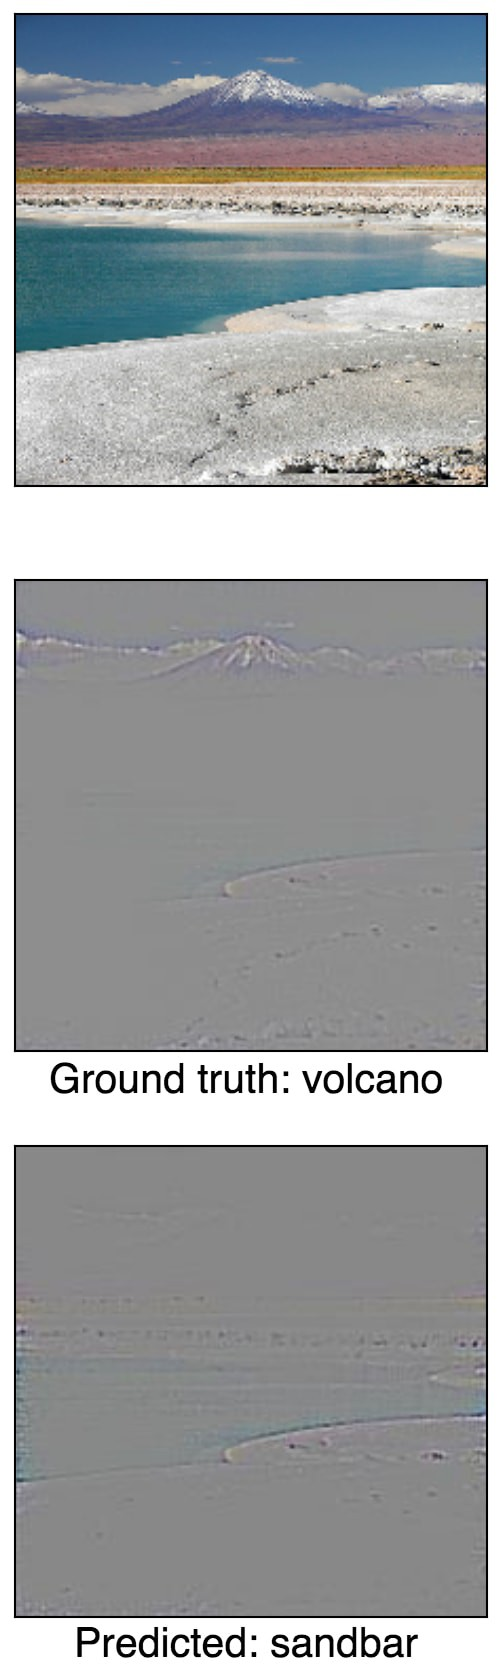
\includegraphics[width=1\linewidth]{figures/failure_62.jpg}
        \caption{}
        \label{fig:failure_volcano}
    \end{subfigure}
    ~
    \begin{subfigure}[b]{0.23\linewidth}
        \centering
        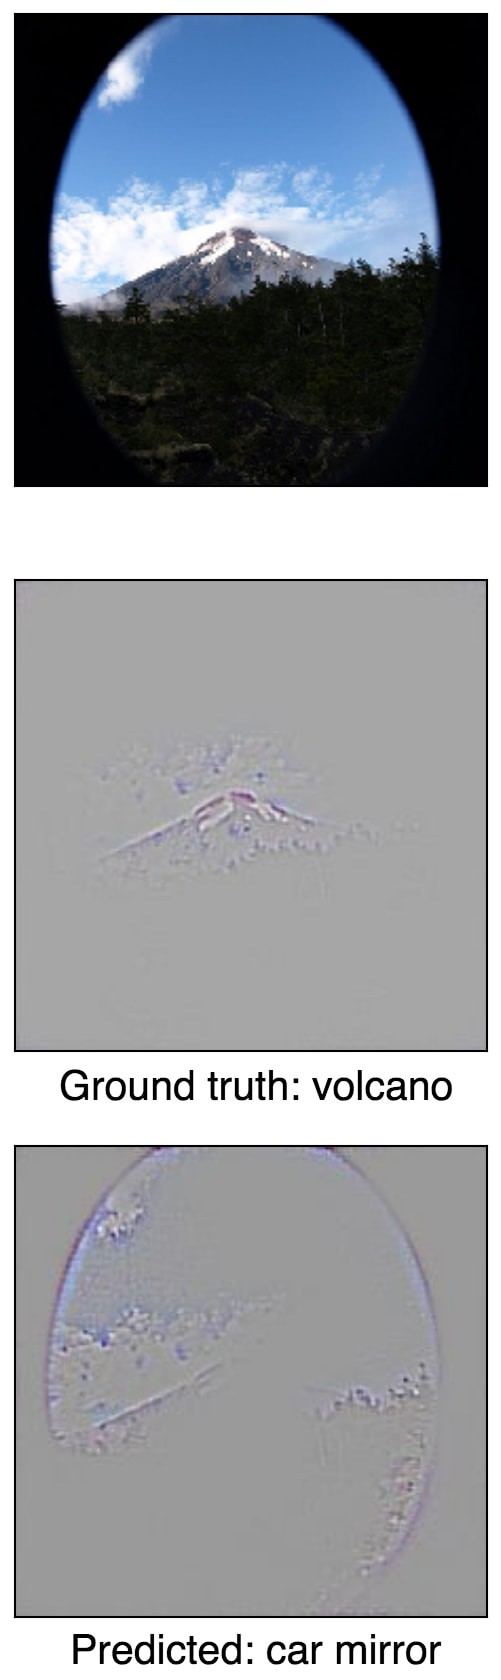
\includegraphics[width=1\linewidth]{figures/failure_11.jpg}
        \caption{}
        \label{fig:failure_mirror}
    \end{subfigure}
    \begin{subfigure}[b]{0.23\linewidth}
        \centering
        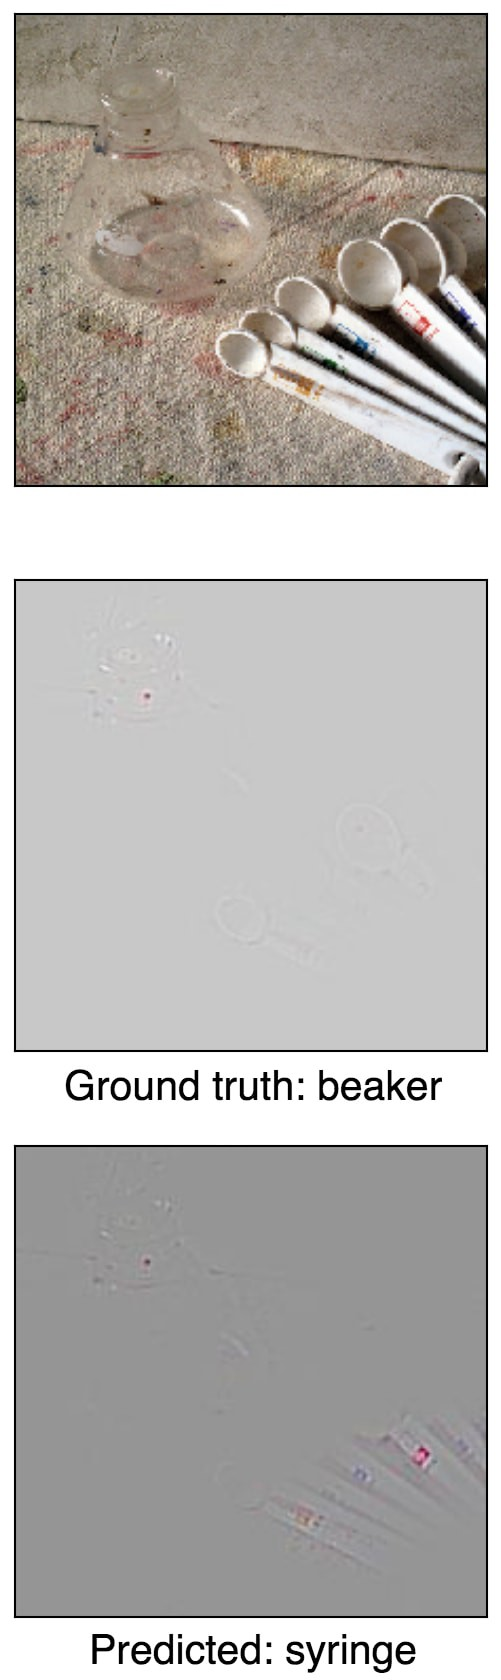
\includegraphics[width=1\linewidth]{figures/failure_60.jpg}
        \caption{}
        \label{fig:failure_syringe}
    \end{subfigure}
    \begin{subfigure}[b]{0.23\linewidth}
        \centering
        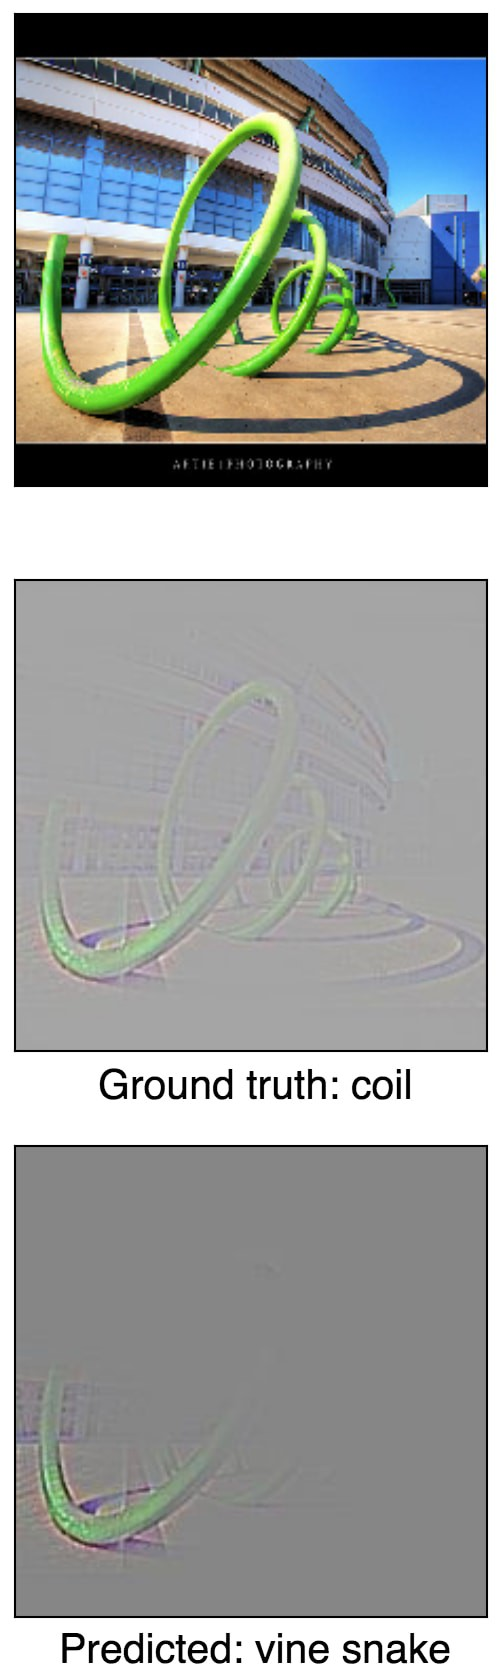
\includegraphics[width=1\linewidth]{figures/failure_78.jpg}
        \caption{}
        \label{fig:failure_snake}
    \end{subfigure}
    \vspace{14pt}
     \caption{
In these cases the model (VGG-16) failed to predict the correct class in its top 1 (a and d) and top 5 (b and c) predictions. Humans would find it hard to explain some of these predictions without looking at the visualization for the predicted class. But with  \gcam{}, these mistakes seem justifiable.
    }
    \label{fig:failures}
    \end{center}
    \vspace{-5pt}
\end{figure}

In order to see what mistakes a network is making, we first get a list of examples
that the network (VGG-16) fails to classify correctly.
For these misclassified examples, we use \cgb{} to visualize both the correct and the predicted class.
As seen in \figref{fig:failures}, some failures are due to ambiguities inherent
in ImageNet classification. We can also see that \emph{seemingly unreasonable
predictions have reasonable explanations}, an
observation also made in HOGgles~\cite{vondrick_iccv13}.
    A major advantage of \cgb{} visualizations over other methods is that due to
    its high-resolution and ability to be class-discriminative, it readily enables these analyses.

\vspace{-8pt}
\subsection{Effect of adversarial noise on VGG-16}\label{sec:adversarial_noise}

Goodfellow \etal~\cite{goodfellow2015explaining} demonstrated the
vulnerability of current deep networks to adversarial examples, which
are slight imperceptible perturbations of input images that fool the network into
misclassifying them with high confidence. We generate adversarial
images for an ImageNet-pretrained VGG-16 model such that it assigns high probability
($>0.9999$) to a category that is not present in the image and low probabilities
to categories that are present. We then compute
\gcam{} visualizations for the categories that are present.
As shown in \reffig{fig:adversarial_main}, despite the network
being certain about the absence of these categories (`tiger cat' and `boxer'),
\gcam{} visualizations can correctly localize them.
This shows that \gcam{} is fairly robust to adversarial noise.
\begin{figure}[ht!]
\vspace{-2pt}
  \begin{center}
    \begin{subfigure}[b]{0.32\linewidth}
        \centering
        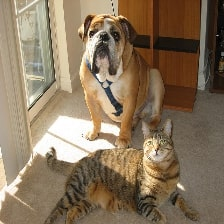
\includegraphics[width=1\linewidth]{figures/caffe2_figs/vgg_orig_cat_dog.jpg}
        \tiny{Boxer: 0.4   Cat: 0.2} %
		\caption{\tiny{Original image}}

        \label{fig:orig_cat_dog}
    \end{subfigure}
    \begin{subfigure}[b]{0.32\linewidth}
        \centering
        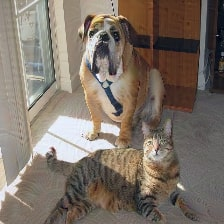
\includegraphics[width=1\linewidth]{figures/caffe2_figs/pos_vgg_405_4_cat_dog.jpg}
        \tiny{Airliner: 0.9999\\
        }
		\caption{\tiny{Adversarial image}}
        \label{fig:adv_cat_dog_airliner}
    \end{subfigure}
    \begin{subfigure}[b]{0.32\linewidth}
        \centering
        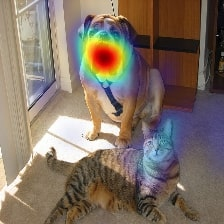
\includegraphics[width=1\linewidth]{figures/gcam_pos_vgg_405_cat_dog_243.jpg}
        \tiny{Boxer: 1.1e-20}
		\caption{\tiny{\gcam{} ``Dog''}}
        \label{fig:gcam_dog_airliner}
    \end{subfigure}
    
    \begin{subfigure}[b]{0.32\linewidth}
    \vspace{10pt}
        \centering
        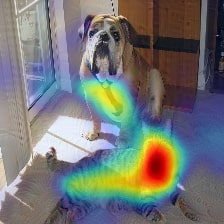
\includegraphics[width=1\linewidth]{figures/gcam_pos_vgg_405_4_cat_dog_283.jpg}
        \tiny{Tiger Cat: 6.5e-17\\}
		\caption{\tiny{\gcam{} ``Cat''}}
        \label{fig:gcam_cat_airliner}
	\end{subfigure}
    \begin{subfigure}[b]{0.33\linewidth}
    \vspace{10pt}
        \centering
        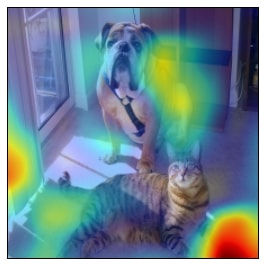
\includegraphics[width=1\linewidth]{figures/caffe2_figs/gcam_pos_vgg_airliner_405.jpg}
        \tiny{Airliner: 0.9999\\}
		\caption{\tiny{\gcam{} ``Airliner''}}
        \label{fig:gcam_airliner_airliner}
	\end{subfigure}
    \begin{subfigure}[b]{0.33\linewidth}
    \vspace{10pt} 
        \centering
        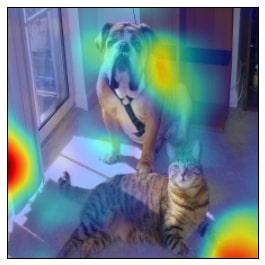
\includegraphics[width=1\linewidth]{figures/caffe2_figs/gcam_pos_vgg_airliner_813.jpg}
        \tiny{Space shuttle: 1e-5\\}
		\caption{\tiny{\gcam{} ``Space Shuttle''}}
        \label{fig:gcam_spaceshuttle_airliner}
	\end{subfigure}
	\vspace{14pt}
	\caption{\rp{
	  (a-b) Original image and the generated adversarial image for
	  category ``airliner''. (c-d) \gcam{} visualizations for the
	  original categories ``tiger cat'' and ``boxer (dog)'' along with their confidence. Despite the network being completely fooled into predicting the dominant category label of
	  ``airliner'' with high confidence (>0.9999), \gcam{} can localize the original categories accurately. \rpi{(e-f) \gcam{} for the top-2 predicted classes ``airliner'' and ``space shuttle'' seems to highlight the background.}}
    }
    \label{fig:adversarial_main}
    \end{center}
\end{figure}

\vspace{-20pt}
\subsection{Identifying bias in dataset}\label{sec:bias}
In this section, we demonstrate another use of \gcam{}: identifying and
reducing bias in training datasets. Models trained on biased datasets may not
generalize to real-world scenarios, or worse, may perpetuate biases and stereotypes
(\wrt gender, race, age, \etc). %
We finetune an ImageNet-pretrained VGG-16 model for a ``doctor'' \vs ``nurse''
binary classification task. We built our training and validation splits using
the top $250$ relevant images (for each class) from a popular image search engine.
And the test set was controlled to be balanced in its distribution
of genders across the two classes. Although the trained model achieves good validation
accuracy, it does not generalize well ($82$\% test accuracy).


\gcam{} visualizations of the model predictions (see the red box\footnote{The green and red boxes are drawn manually to highlight correct and incorrect focus of the model.} regions in the middle column of \reffig{fig:bias_qual})
revealed that the model had learned to look at the person's face / hairstyle to distinguish nurses from doctors, thus learning a gender stereotype.
Indeed, the model was misclassifying several female doctors to be a nurse and male nurses to be a doctor. Clearly, this is problematic. Turns out the image search results were gender-biased (78\% of images for doctors were men, and 93\% images for nurses were women).

\begin{figure}[htp]
 \centering
 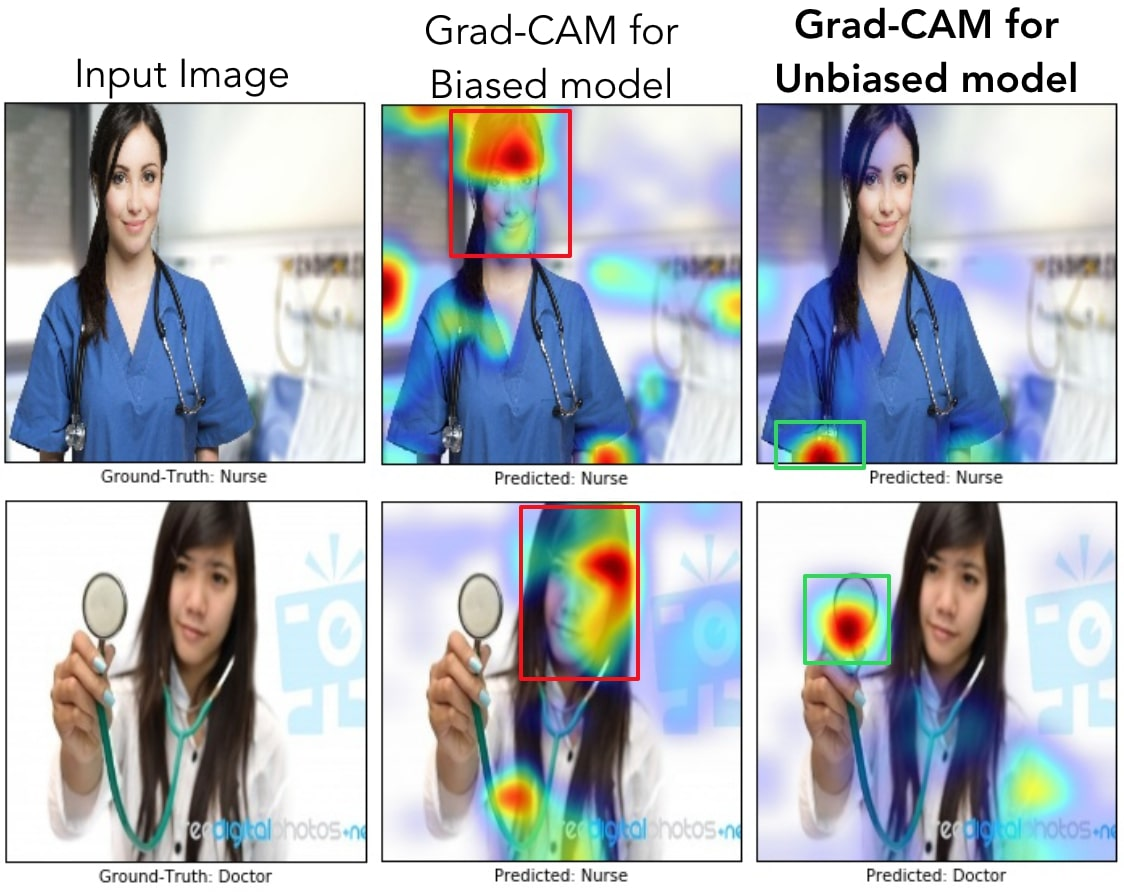
\includegraphics[width=1\linewidth]{figures/bias_qualitative.jpg}
 \caption{In the first row, we can see that even though both models made the right decision, the biased model (model1) was looking at the face of the person to decide if the person was a nurse, whereas the unbiased model was looking at the short sleeves to make the decision. For the example image in the second row, the biased model made the wrong prediction (misclassifying a doctor as a nurse) by looking at the face and the hairstyle, whereas the unbiased model made the right prediction looking at the white coat, and the stethoscope.
 }
 \label{fig:bias_qual}
\end{figure}

Through these intuitions gained from \gcam{} visualizations,
we reduced bias in the training set by adding in images of male nurses and female doctors,
while maintaining the same number of images per class as before.
The re-trained model not only generalizes better ($90$\% test accuracy),
but also looks at the right regions (last column of \reffig{fig:bias_qual}).
This experiment demonstrates a proof-of-concept that \gcam{} can help detect and
remove biases in datasets, which is important not just for better generalization,
but also for fair and ethical outcomes as more algorithmic decisions are made in society.





